\subsubsection{PWM module}
\label{sec:pwm}
Each phase of the inverter is controlled by a PWM signal for its high-side leg and one for its low-side leg. 

The module shown on figure \ref{fig:pwm_module} is made to control both the high-side and low-side transistors of a leg in the inverter. Three instances of the module is used to control all three phases.
\begin{figure}[H]
	\centering
	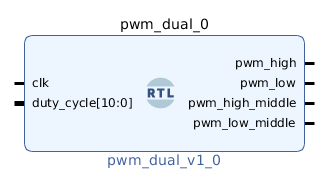
\includegraphics[width=0.5 \textwidth]{pictures/software/pwm_module.png}
	\caption{The PWM module made to control both high-side and low-side transistors of a leg in the inverter.}
	\label{fig:pwm_module}
\end{figure}



\subsubsection*{Counter}
A counter is used for implementing the PWM. For every rising edge of the input clock the counter takes one step up or down depending on its current counting direction. When it reaches one of its outer limits the counting direction is switched as can be seen on figure \ref{fig:counter}.

\begin{figure}[H]
	\centering
	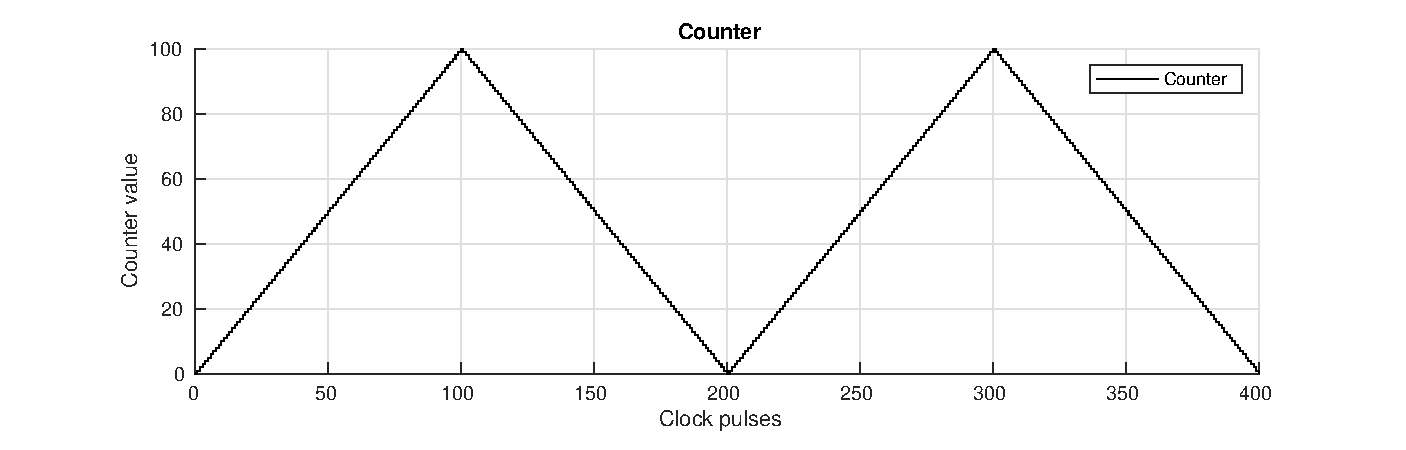
\includegraphics[width=1 \textwidth]{pictures/software/counter.eps}
	\caption{How the counter is counted up and down over time.}
	\label{fig:counter}
\end{figure}

The resolution of the PWM duty cycle is $1\%$ which means the counter should take $100$ steps from minimum to maximum. The PWM is made as a phase correct PWM and therefore the counter counts both up and down per period this results in $200$ steps per period. 

The signal out of the PWM generator should be the same frequency as the inverter components are designed for in the earlier sections which is $10kHz$. The input clock is already prescaling the output frequency by the number of counter steps but this is not enough and therefore in order for the PWM to have the correct frequency an additional prescaler is added. The prescaler value is found with equation \ref{eq:additional_prescaler}.

The prescaler will be made with a counter that counts up to some value, $x$. When the value is reached the output clock is flipped and the counter is reset. Such a prescaler has a build in prescaling of 2 which is added besides the additional prescaler leading to equation \ref{eq:additional_prescaler1}.



\begin{subequations}
    \begin{align}
        \begin{split}
            fs = \frac{clk}{steps \cdot x \cdot 2}
            \label{eq:additional_prescaler1}
        \end{split} \\ 
        \begin{split}
             x = \frac{clk}{fs \cdot steps \cdot 2}
        \end{split} \\ 
        \begin{split}
            x = \frac{125MHz}{10kHz \cdot 200 \cdot 2} = 31.25 \sim 31
            \label{eq:additional_prescaler}
        \end{split} \\
        \begin{split}
            \frac{125MHz}{200 \cdot 31 \cdot 2} = 10.08kHz
        \end{split}
    \end{align}
\end{subequations}

Where $fs$ is the output frequency of the PWM signal, $steps$ is the number of counter steps in a period, $clk$ is the input clock which in this case is the internal $125MHz$ clock and $x$ is the additional prescaler.

With the additional prescaler the PWM module outputs PWM signals with a frequency of $10.08kHz$.

\subsubsection*{PWM}


To handle both a high-side PWM and low-side PWM each of the signals have a threshold and the output signal changes from high to low or opposite when the counter crosses the threshold as can be seen in figure \ref{fig:counter_with_pwm}. The two thresholds are spaced out with a static dead time between them which is discussed later in this section. The dead time on figure \ref{fig:counter_with_pwm} has been exaggerated to make it more visible.

\begin{figure}[H]
	\centering
	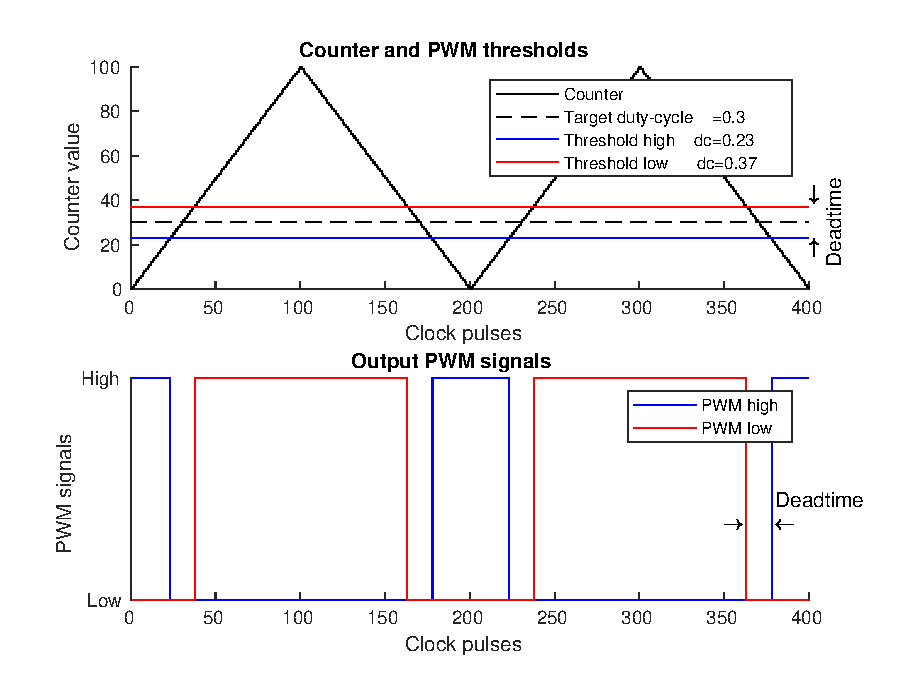
\includegraphics[width=0.8 \textwidth]{pictures/software/counter_with_pwm.eps}
	\caption{The top shows the target duty-cycle together with the thresholds compared to the PWM counter. The bottom shows the output PWM signals. The dead time is exaggerated to make it more visible.}
	\label{fig:counter_with_pwm}
\end{figure}

The high-side PWM is high when the counter is below the high-side threshold, $counter < th_{high}$, otherwise it is low. 

The low-side PWM is high when the counter is above the low-side threshold, $counter > th_{low}$ otherwise it is low.

The VHDL code can be seen below.

\begin{minted}[frame=single,framesep=2mm,baselinestretch=1.2,linenos,fontsize=\footnotesize]{vhdl}
-- Control of the high side PWM
pwm_high <= HIGH when (counter < threshold_high) else LOW;
-- Control of the low side PWM
pwm_low  <= HIGH when (counter > threshold_low) else LOW;
\end{minted}
\begin{center}
    The VHDL code to control the PWM signals.
\end{center}


To avoid shorting the supply dead time is inserted between turning off one transistor and turning on the other.

On figure \ref{fig:turn_off_time1} the conducted current for each transistor is drawn next to the PWM signals with dead time being bigger than the transistor turn off time, $dead \ time > t_{turn \ off}$, which results in one transistor turning completely off before the other turns on. 

\begin{figure}[H]
	\centering
	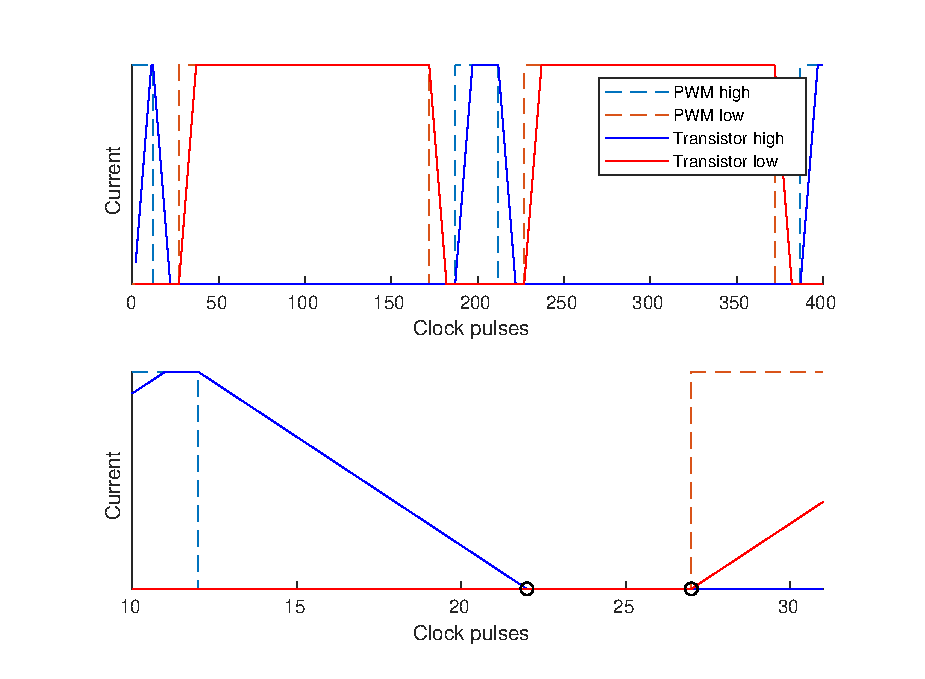
\includegraphics[width=0.8 \textwidth]{pictures/software/turn_off_time1.eps}
	\caption{PWM with dead time and transistor conduction curves for systems with $dead \ time > t_{turn \ off}$}
	\label{fig:turn_off_time1}
\end{figure}

On figure \ref{fig:turn_off_time2} the conducted current for each transistor is drawn next to the PWM signals but this time the dead time is smaller than the transistor turn off time, $dead \ time < t_{turn \ off}$, which results in both transistors conducting at the same time.
When both transistors conduct the supply is shorted which should be avoided especially when the supply consist of batteries.

\begin{figure}[H]
	\centering
	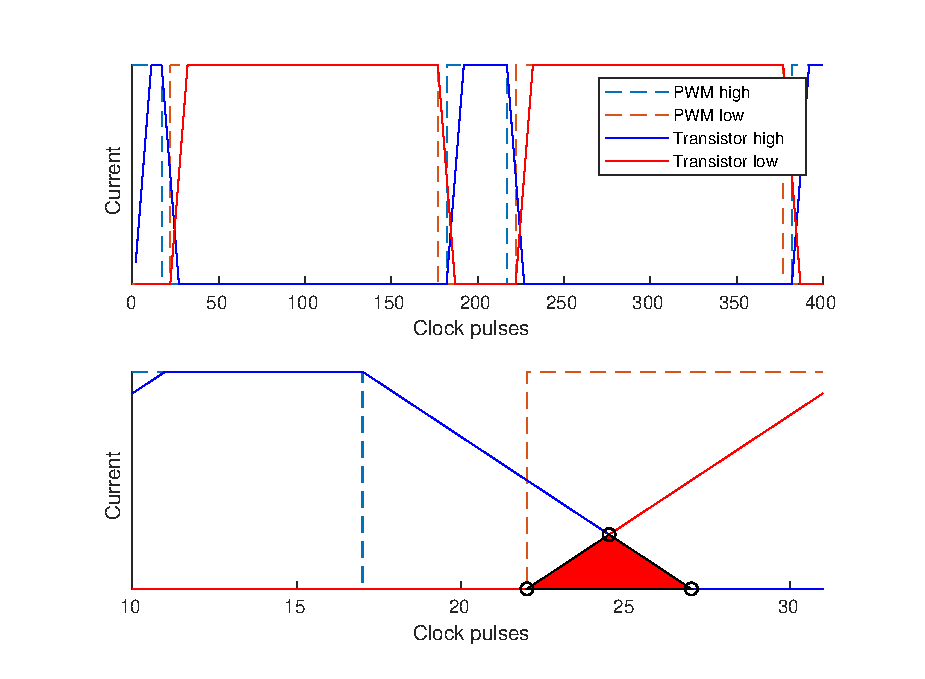
\includegraphics[width=0.8 \textwidth]{pictures/software/turn_off_time2.eps}
	\caption{PWM with dead time and transistor conduction curves for systems with $dead \ time < t_{turn \ off}$}
	\label{fig:turn_off_time2}
\end{figure}

It is therefore important to choose the dead time big enough to avoid shorting but also not so big that the systems performance is unnecessarily reduced.

To avoid compromising the required dead time at edge cases where one of the thresholds tries to move above $100 \%$ or  below $0 \%$ the thresholds are found in two different ways.





When the high-side threshold is greater than the counter minimum plus half of the dead time it is placed half of the dead time below the threshold.
\begin{equation}
    th_{duty \ cycle} \geq  counter_{min} + \frac{t_{dead \ time}}{2}
    \label{eq:threshold_high_condition}
\end{equation}
\begin{center}
    $\Downarrow$    
\end{center}
\begin{equation}
   th_{high} = th_{duty \ cycle} - \frac{t_{dead \ time}}{2}  
   \label{eq:threshold_high_equation}
\end{equation}

Otherwise the threshold is clamped to the counter bottom edge $th_{high} = counter_{min}$ which is possible because the PWM is switched when $th_{high} > counter$.
If the threshold comes too close to the edge the threshold will be clamped and the PWM will not switch. Had the PWM being switched when $th_{high} \geq counter$ this would not have worked.



The low-side threshold is placed half of the dead time above the threshold when the duty cycle is at least half of the dead time below the counter max.
\begin{equation}
    th_{duty \ cycle}\leq counter_{max} - \frac{t_{dead \ time}}{2}
    \label{eq:threshold_low_condition}
\end{equation}
\begin{center}
    $\Downarrow$
\end{center}
\begin{equation}
  th_{low} = th_{duty \ cycle} + \frac{t_{dead \ time}}{2}  
  \label{eq:threshold_low_equation}
\end{equation}
Otherwise the threshold is clamped to the top counter edge.

The VHDL code to find the two thresholds can be seen below. The variable \textit{duty\textunderscore cycle} is parsed into the PWM module from the higher level control. \textit{DEADTIME}, \textit{HALF\textunderscore DEADTIME}, \textit{COUNT\textunderscore MIN} and \textit{COUNT\textunderscore MAX} are all constants.

\begin{minted}[frame=single,framesep=2mm,baselinestretch=1.2,linenos,fontsize=\footnotesize]{vhdl}
-- Get half of dead time
HALF_DEADTIME(6 downto 0) <= DEADTIME(7 downto 1);
-- Find the threshold for the high-side PWM
threshold_high <= duty_cycle - HALF_DEADTIME when 
                (duty_cycle >= COUNT_MIN + HALF_DEADTIME) else COUNT_MIN;
-- Find the threshold for the low-side PWM
threshold_low  <= duty_cycle + HALF_DEADTIME when 
                (duty_cycle <= COUNT_MAX - HALF_DEADTIME) else COUNT_MAX;
\end{minted}
\begin{center}
    The VHDL code to find the thresholds for the high and low side PWM signals. The conditions and equations used are \ref{eq:threshold_high_condition}, \ref{eq:threshold_high_equation}, \ref{eq:threshold_low_condition} and \ref{eq:threshold_low_equation}.
\end{center}



The turn off times for the transistors used in the inverter are $50ns$ as discussed in section \todo{Refer to section}. 
The way dead time is implemented it has to be defined as some even amount of ticks at the PWM frequency.
The minimum dead time step, $dt_{res}$, in this system is calculated with equation \ref{eq:minimum_deadtime_resolution}.

\begin{subequations}
    \begin{align}
        \begin{split}
            dt_{res} = \frac{T}{2} \cdot \frac{dt_{min}}{counter_{max}}
        \end{split} \\ 
        \begin{split}
             dt_{res} = \frac{2}{fs} \cdot \frac{dt_{min}}{counter_{max}}
        \end{split} \\ 
        \begin{split}
             dt_{res} = \frac{2}{10kHz} \cdot \frac{2}{100} = 1\mu s
        \end{split} 
    \end{align}
    \label{eq:minimum_deadtime_resolution}
\end{subequations}

Which gives the system a safety margin of $20$ on the dead time between the two PWM signals.


\subsubsection*{ADC Pulses}

To trigger a new reading by the ADC the PWM generator module has a build-in pulse mechanism that outputs a pulse in the middle of each of the PWM periods as can be seen on figure \ref{fig:adc_pulses}. The pulse in the middle of the high-side PWM is used to trigger the ADC.

\begin{figure}[H]
	\centering
	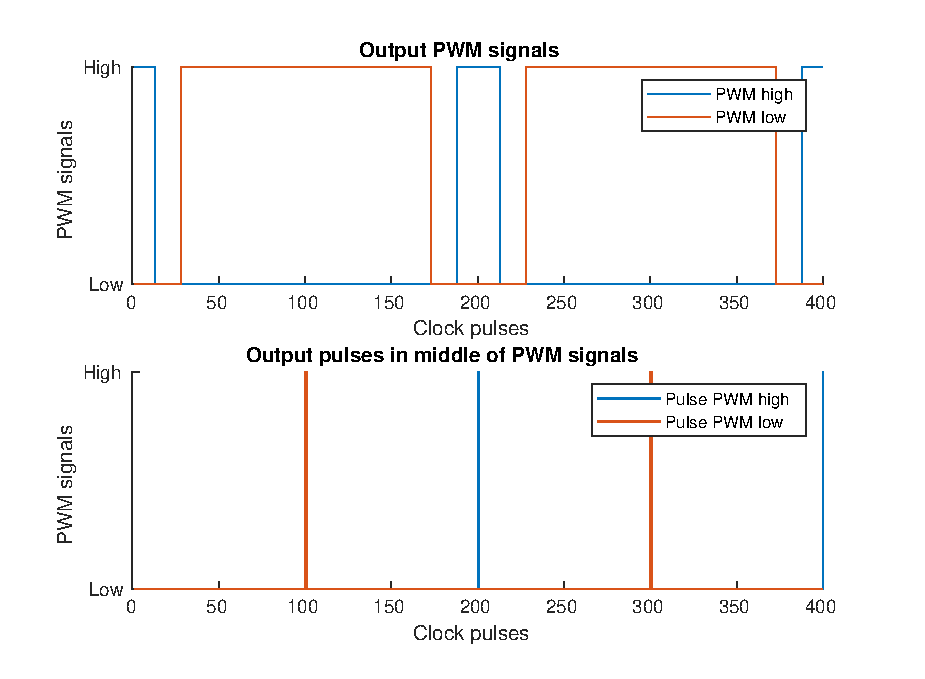
\includegraphics[width=0.8 \textwidth]{pictures/software/adc_pulses.eps}
	\caption{The top graph shows the high and low side PWM signals. The bottom graph shows the ADC pulses triggered in the middle of each PWM signal.}
	\label{fig:adc_pulses}
\end{figure}

The code for evaluating the signal states can be seen below. The code utilizes the concurrent nature of VHDL which makes it fast and robust.
When the counter reaches its bottom edge the high pulse is set high and as soon as the counter starts going up again the signal is set low. The low pulse is controlled in the same way but this happens at the high counter edge instead.

\begin{minted}[frame=single,framesep=2mm,baselinestretch=1.2,linenos]{vhdl}
-- Output a pulse in the middle of the high PWM signal
pwm_high_middle <= HIGH when (counter <= COUNT_MIN) else LOW;

-- Output a pulse in the middle of the low PWM signal
pwm_low_middle <= HIGH when (counter >= COUNT_MAX) else LOW;
\end{minted}
\begin{center}
    The VHDL code to control the ADC pulses.
\end{center}


\subsubsection*{Test of PWM module}

To test the PWM generators a test scenario is set up. A simulated rotor angle and simulated currents are parsed into the control system and the outputs are measured with an oscilloscope. 
The maximum sine frequency expected out of the system is $333Hz$. To figure out how fast the simulated angle should change the time between each angle change is found. 
The angle is chosen to with $1$ degree steps. That gives a change rate of:


\begin{equation}
    change_{rate} = sin_{freq} \cdot 360^o
\end{equation}
Where $sin_{freq}$ is the target sine frequency. Which results in a time per angle of
\begin{equation}
    t_{angle} = \frac{1}{change_{rate}} = \frac{1}{333Hz \cdot 360^o} = 8 \mu s
\end{equation}
Where $t_{angle}$ is the time per angle. 

No currents will run in the system so the currents need to be simulate as well. The angle is used to calculate three sinusoidal curves. The way the three currents are calculated can be seen in equation \ref{eq:simulated_currents}.

\begin{equation}
    i_A = sin(angle), \ \ i_B = sin(angle + 120^o), \ \ i_C = sin(angle + 240^o)
    \label{eq:simulated_currents}
\end{equation}


Implementing this gives the PWM signal on one of the phases as seen in the top of figure \ref{fig:one_phase} and the resulting sine curve on the bottom.

\begin{figure}[H]
	\centering
	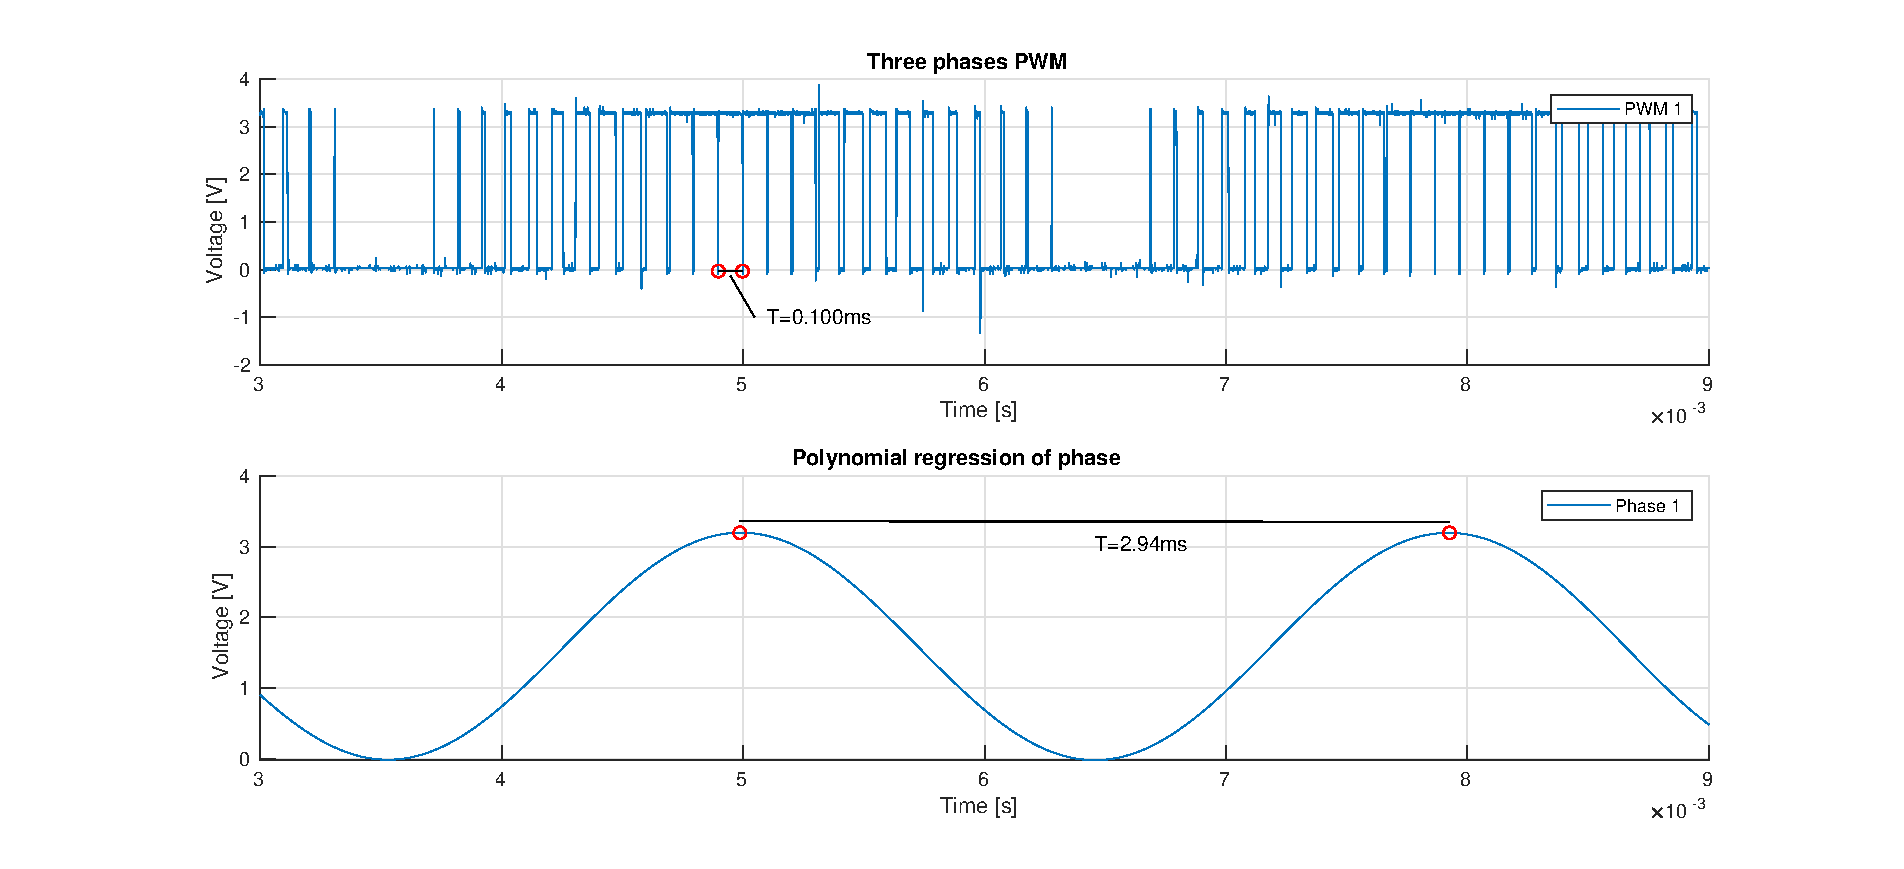
\includegraphics[width=1 \textwidth]{pictures/software/one_phase.eps}
	\caption{Testing of one phase. The top graph shows the PWM signals. The bottom graph shows the resulting sine curve found with a polynomial regression.}
	\label{fig:one_phase}
\end{figure}

The PWM frequency can be found by measuring the time between the middle of two PWM periods as can be seen in equation \ref{eq:pwm_frequency}. 
\begin{equation}
    PWM_{freq} = \frac{1}{0.100 \cdot 10^{-3}} = 10kHz
    \label{eq:pwm_frequency}
\end{equation}
With a precision of 6 decimals on the time period the frequency of the PWM signal turns out to be $10kHz$.

The resulting sine can be found by applying a polynomial regression to the PWM signal which results in a sinusoidal curve. The frequency is found from the inverse of the time period between two points exactly one period apart. 
\begin{equation}
    sin_{freq} = \frac{1}{2.94 \cdot 10^{-3}} = 340 Hz
\end{equation}
The frequency of the sine is $340Hz$.

On figure \ref{fig:one_phase} only one of the phases are shown. In reality the system outputs three phases and all can be seen on figure \ref{fig:three_phases}. The periods in between the peak of the three phases are shown to determine the amount of phase shift. The time of one third of a period is calculated with \ref{eq:one_third_period}-
\begin{equation}
    \frac{1}{3} \cdot \frac{1}{340} = 0.9804ms
    \label{eq:one_third_period}
\end{equation}
By comparing the theoretical and measured periods between the phases it is determined that the phases are phase shifted with approximately $120^o = 2 \pi / 3 \ rad$.
\begin{figure}[H]
	\centering
	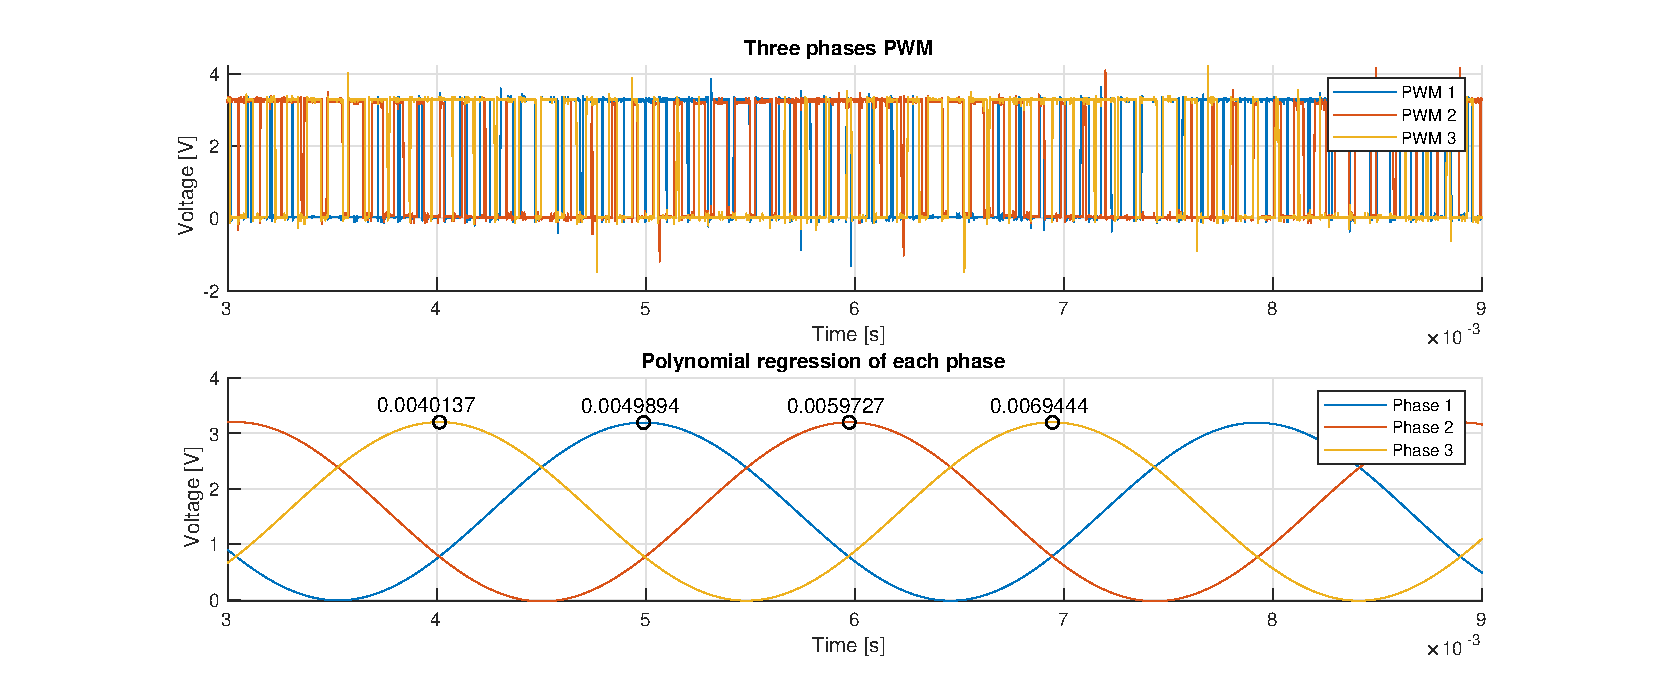
\includegraphics[width=1 \textwidth]{pictures/software/three_phases.eps}
	\caption{Testing of all three phases. The top graph shows the PWM signals. The bottom graph shows the resulting sine curves found with polynomial regressions.}
	\label{fig:three_phases}
\end{figure}
